% File: chapters/chapter1_introduction.tex

\chapter{Introduction}
\label{chap:introduction}

\section{Background and Motivation}
\label{sec:background_motivation}

Automotive software has changed fundamentally in the last 15 years. When I first read about vehicle cybersecurity, I was surprised to learn that a modern car runs over 100 million lines of code. Not thousands. Not millions. Over 100 million. Distributed across more than 100 Electronic Control Units (ECUs). This number, which appears in industry reports \cite{Charette2009, Broy2006}, illustrates a complete shift in how we think about vehicles.

This shift came from somewhere. Vehicles used to be mechanical systems. An engine controller managed fuel injection. An ABS system prevented wheel lockup. These systems mostly operated independently. A skilled engineer could understand the complete electronic architecture within weeks. That is gone now.

Today, vehicles are software platforms that happen to have wheels. Tesla demonstrated this most clearly. When Tesla updates a vehicle over the air, customers receive new features, better performance, and improved safety. All without visiting a service center. Traditional automakers watched this happen and realized something fundamental had changed. Software now determines competitive advantage. It determines how fast a car accelerates. It determines what features customers receive. Mechanical engineering no longer drives differentiation.

This transformation created a problem. Software is complex. A single vehicle contains code spanning multiple programming paradigms, different safety criticality levels, and various execution environments. Code that is safety-critical on AUTOSAR platforms follows entirely different development rules than infotainment applications running on Linux. Real-time control systems operating at microsecond intervals coexist with cloud-connected services. This diversity makes testing exponentially harder.

Consider a Level 2 automated driving system. Perception algorithms process camera, radar, and lidar data. Planning modules compute safe trajectories. Control systems translate trajectories into steering and throttle commands. Each layer requires different technical expertise: computer vision, machine learning, control theory, real-time systems. Integration alone consumes enormous effort. When you add legacy code to this, code written years ago with minimal documentation, understanding what the software actually does becomes detective work.

\subsection{Security Challenges in Modern Systems}
\label{sec:security_challenges}

This complexity creates security risks that are genuinely dangerous. When a web server gets compromised, the consequences are serious. Data theft, service disruption, financial loss. When a vehicle control system is compromised, it can result in severe physical harm or fatal injuries. This is not theoretical. In 2015, researchers demonstrated remote exploitation of a Jeep Cherokee. They showed scenarios where attackers could disable brakes or seize steering at highway speeds \cite{MillerValasek2015}. Chrysler recalled 1.4 million vehicles. The infotainment system, connected via cellular networks, had provided a pathway to safety-critical networks.

Regulators noticed a critical security gap in vehicle software. UNECE Regulation 155 now requires cybersecurity management systems for all new vehicle types \cite{UNECER155}. ISO/SAE 21434 sets cybersecurity engineering requirements across the entire vehicle lifecycle \cite{ISO21434}. These are not suggestions. Vehicles that do not comply cannot be sold in regulated markets. Manufacturers must demonstrate that security was designed into systems from the beginning, not bolted on afterward.

This regulatory pressure collides with a fundamental tension in automotive security testing. Safety-critical systems undergo exhaustive verification against precisely defined requirements, like ISO 26262 \cite{ISO26262}. Every possible failure mode is analyzed. Fixes are tested. This works for safety, where hazards are known and physics are deterministic.

Security is different. The adversary is intelligent, creative, and unconstrained by specifications. Attackers do not limit themselves to documented interfaces. They probe for implementation weaknesses, logic errors, overlooked edge cases. Testing for security means exploring the unexpected, not verifying the expected. This requires fundamentally different approaches.

\subsection{Fuzzing}
\label{sec:fuzzing}

\begin{figure}[htbp]
    \centering
    \resizebox{\textwidth}{!}{
    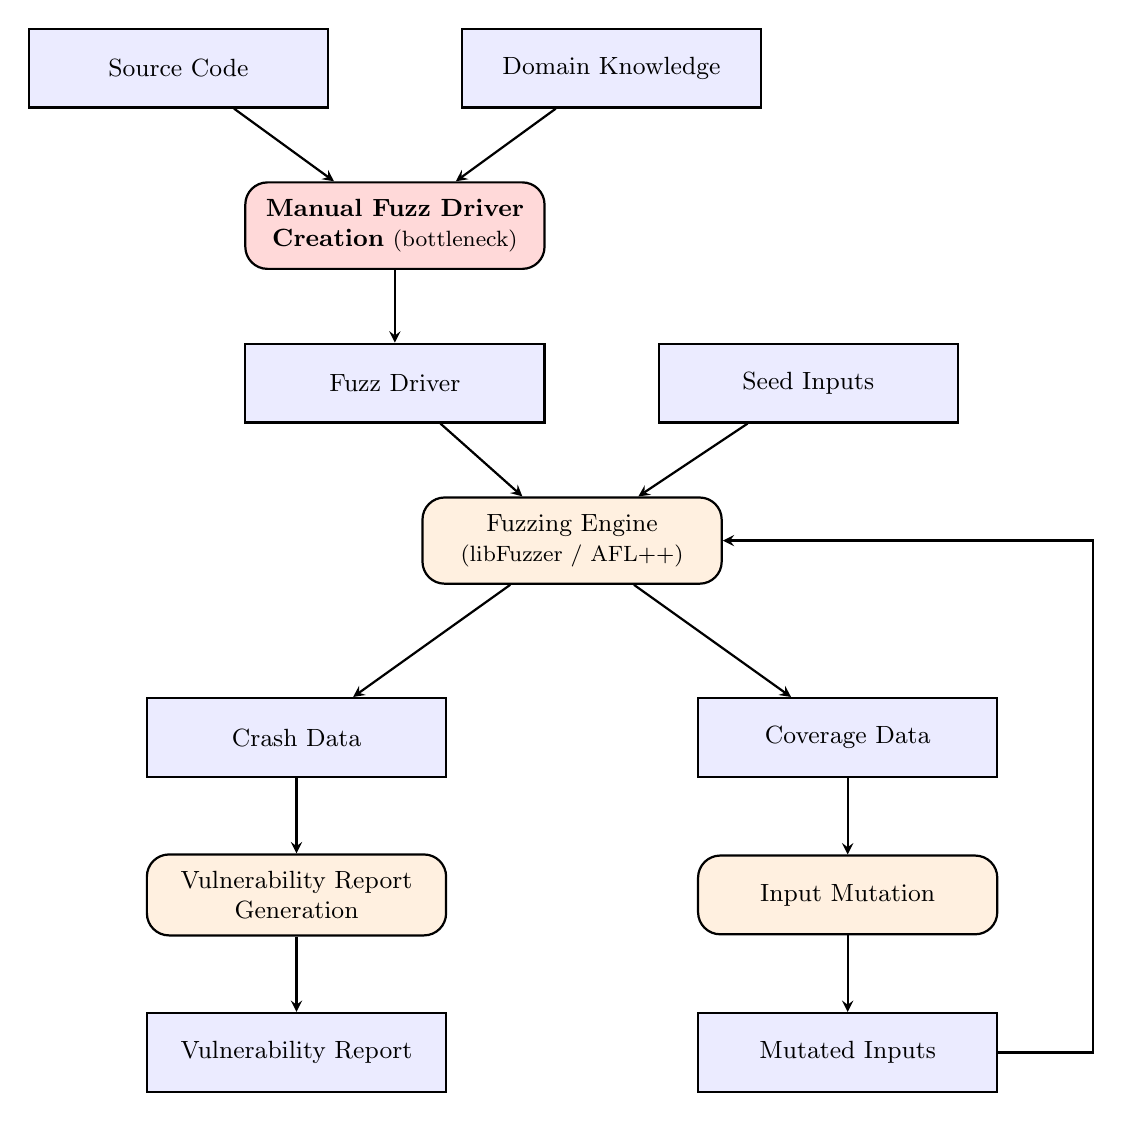
\begin{tikzpicture}[
        databox/.style={draw, rectangle, minimum width=3.8cm, minimum height=1cm, align=center, fill=blue!8, thick, font=\small},
        procbox/.style={draw, rounded corners=8pt, rectangle, minimum width=3.8cm, minimum height=1cm, align=center, fill=orange!12, thick, font=\small},
        arrow/.style={->, >=stealth, thick},
        every node/.style={inner sep=6pt}
    ]
    % --- ROW 1: Developer inputs ---
    \node[databox] (srccode) at (0,0) {Source Code};
    \node[databox] (domknow) at (5.5,0) {Domain Knowledge};

    % --- ROW 2: Manual driver writing (bottleneck) ---
    \node[procbox, fill=red!15] (driverwrite) at (2.75,-2) {\textbf{Manual Fuzz Driver}\\\textbf{Creation} {\footnotesize(bottleneck)}};

    % --- ROW 3: Fuzz Driver ---
    \node[databox] (fuzzdriver) at (2.75,-4) {Fuzz Driver};
    \node[databox] (seedinputs) at (8,-4) {Seed Inputs};

    % --- ROW 4: Fuzzing Engine ---
    \node[procbox] (fuzzengine) at (5,-6) {Fuzzing Engine\\{\footnotesize(libFuzzer / AFL++)}};

    % --- ROW 5: Outputs ---
    \node[databox] (crashdata) at (1.5,-8.5) {Crash Data};
    \node[databox] (covdata) at (8.5,-8.5) {Coverage Data};

    % --- ROW 6: Processing ---
    \node[procbox] (vuln) at (1.5,-10.5) {Vulnerability Report\\Generation};
    \node[procbox] (mutate) at (8.5,-10.5) {Input Mutation};

    % --- ROW 7: Final outputs ---
    \node[databox] (vulnreport) at (1.5,-12.5) {Vulnerability Report};
    \node[databox] (mutinputs) at (8.5,-12.5) {Mutated Inputs};

    % --- ARROWS ---
    \draw[arrow] (srccode) -- (driverwrite);
    \draw[arrow] (domknow) -- (driverwrite);
    \draw[arrow] (driverwrite) -- (fuzzdriver);
    \draw[arrow] (fuzzdriver) -- (fuzzengine);
    \draw[arrow] (seedinputs) -- (fuzzengine);
    \draw[arrow] (fuzzengine) -- (crashdata);
    \draw[arrow] (fuzzengine) -- (covdata);
    \draw[arrow] (crashdata) -- (vuln);
    \draw[arrow] (covdata) -- (mutate);
    \draw[arrow] (vuln) -- (vulnreport);
    \draw[arrow] (mutate) -- (mutinputs);

    % --- Feedback loop ---
    \draw[arrow] (mutinputs.east) -- ++(1.2,0) |- (fuzzengine.east);

    \end{tikzpicture}
    }
    \caption{The Fuzzing Process. Data artifacts are shown in rectangular boxes; processing steps are shown in rounded boxes. The manual creation of fuzz drivers (highlighted in red) is the bottleneck this thesis aims to automate.}
    \label{fig:fuzzing_concept}
\end{figure}

The fuzzing architecture begins with the human element. The developer writes the initial source code and possesses the critical domain knowledge required to understand the intended software logic. Because an automated system cannot inherently know what specific areas to target, the developer must manually define the testing scope and create the fuzz driver, a small program that translates raw fuzzer inputs into meaningful API calls. This manual creation step requires significant effort and specialized expertise, representing the primary bottleneck that this research aims to automate.

Once the fuzz driver and seed inputs are supplied, the automated fuzzing engine takes control. As illustrated in Figure~\ref{fig:fuzzing_concept}, the engine continuously executes the fuzz driver against the target software, feeding it generated inputs while actively monitoring for unexpected behavior. If a crash is detected, the engine extracts the crash data, and a vulnerability report is generated. Conversely, if the execution completes without error, the engine collects coverage data to understand which code paths were reached. An input mutation step then creates slightly altered variations of the previous inputs. These mutated inputs are fed back into the execution loop, driving a continuous cycle of automated vulnerability discovery.


\subsection{CI/CD Pipeline Context}
\label{sec:cicd_context}

Modern software development has embraced a philosophy: integrate code frequently, test automatically, deploy rapidly. The reasoning is sound. Small, incremental changes are easier to understand and debug than large infrequent releases. Automated testing catches regressions before they spread. Fast feedback loops let developers address problems while context is fresh \cite{Humble2010, Fowler2006}.

The automotive industry has adopted these principles, adapting them to domain-specific constraints. You do not casually push untested code to vehicles traveling at highway speeds. Automotive continuous integration pipelines typically feed into formal release processes with human review and additional validation before software reaches production vehicles.

But the core principles hold: automate what you can, test early and often, maintain a continuously releasable codebase \cite{CiCdFuzzing2022}.

\begin{figure}[htbp]
    \centering
    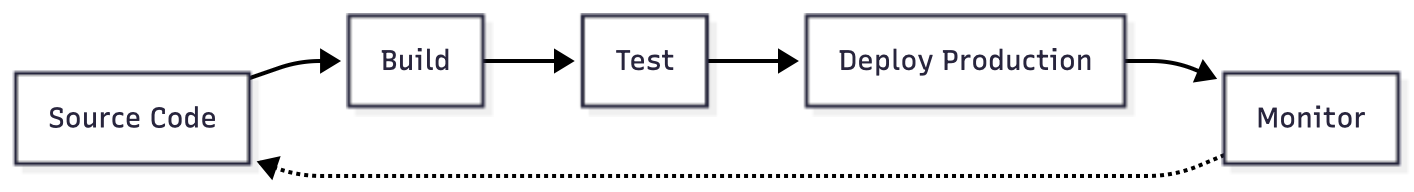
\includegraphics[width=\textwidth]{bilder/cicd.png}
    \caption{The Automotive CI/CD Pipeline. The diagram illustrates the stages from code commit through deployment, highlighting where security validation typically occurs.}
    \label{fig:cicd_pipeline}
\end{figure}

This creates a tension. A well-optimized pipeline might complete build and basic testing in 15 to 30 minutes. Developers expect rapid feedback. But security testing, especially fuzzing, often requires extended execution. A fuzzing campaign might run for hours or days to discover subtle vulnerabilities \cite{OSSFuzzBugs2021}. This timescale is incompatible with developer expectations for fast feedback.

Enterprise environments add additional complexity. Large organizations balance computational demands against security requirements. Build runners may execute in public cloud for scalability while sensitive operations stay in private networks isolated from external connections \cite{AzureDevOps}. Network policies restrict communication between zones. A simple task like calling an LLM API from a build runner encounters firewalls, proxy servers, and access control systems.


\section{Problem Statement}
\label{sec:problem_statement}

The core problem is straightforward: code production vastly outpaces security analysis capacity.

In the broader automotive software industry, massive development teams deploy continuous code modifications. For example, at CARIAD, hundreds of developers produce thousands of changes daily. Even well-staffed security teams cannot review each change for vulnerabilities. Automated tools like SonarQube, Coverity, and Checkmarx provide assistance, but static analysis frequently generates false positives that require manual human triage, and dynamic analysis requires test harnesses that must be created manually.

Fuzzing attempts to bypass this manual review bottleneck, though it introduces a different limitation. Google's OSS Fuzz project has found over 10,000 vulnerabilities in open source software through continuous fuzzing \cite{OSSFuzzBugs2021, LibFuzzer2015}. The effectiveness of this approach is extensively documented. The constraint is fuzz driver creation.

A fuzz driver is a small program that feeds generated inputs to target functionality. Writing effective drivers requires understanding API contracts, identifying interesting code paths, and constructing inputs that explore edge cases. This is specialized work. While the automotive software industry employs specialists capable of writing these drivers, the available workforce cannot scale to match the massive volume of daily code production required by major manufacturers.

The mismatch creates a security gap. Code ships with inadequate fuzzing coverage. Vulnerabilities that could have been discovered through systematic fuzzing remain hidden until attackers find them or security incidents force discovery.

Large Language Models offer a potential solution. These models, trained on vast amounts of source code, can generate syntactically correct code following common patterns \cite{Touvron2023, Bai2023}. Recent research shows LLM capabilities in various software engineering tasks: code completion, bug detection, test generation, documentation \cite{TitanFuzz2022, Fuzz4All2023}.

The question we asked was simple: can LLMs generate fuzz drivers? Specifically, can they generate drivers that compile, execute without crashing, and achieve meaningful code coverage?

This question mattered to us at CARIAD because if the answer was yes, it could change how we approach security testing at scale.

\section{Research Questions and Objectives}
\label{sec:rq_objectives}

We had three main research questions driving this work.

\subsection{Primary Research Questions}
\label{sec:primary_rq}

\textbf{RQ1 (Effectiveness): Can Large Language Models generate fuzz drivers for C++ code that compile successfully, execute without errors, and achieve meaningful code coverage?}

This is the fundamental question. A driver that fails to compile is useless. One that compiles but crashes immediately provides no security value. A driver that runs but only exercises trivial code paths does not justify its existence. Meaningful coverage means reaching error handling paths, boundary conditions, and complex interaction sequences \cite{LLMDriverGenEffectiveness2023}.

\textbf{RQ2 (Optimization): Does model size determine fuzz driver quality, or can smaller models with domain-specific training match or exceed larger general purpose models?}

Everyone in machine learning hears that bigger models are better. Models with more parameters consistently outperform smaller ones on standard benchmarks \cite{Jiang2023}. The largest models show impressive capabilities across diverse tasks. They are also expensive, require substantial compute, and often have rate limits. But domain-specific tuning offers an alternative path \cite{Hu2021}. Instead of relying on the general knowledge of massive models, we adapt smaller models to specific tasks.

We wanted to know: which approach wins for fuzz driver generation?

\textbf{RQ3 (Feasibility): Can LLM-assisted fuzz driver generation be integrated into secure enterprise CI/CD pipelines that are isolated from external networks while meeting performance, cost, and security requirements?}

Academic research often evaluates techniques in isolation, abstracting away deployment concerns. Production matters. Can the solution run within CI/CD time constraints? Does the cost fit budget limits? Can it operate under network security policies that restrict external communication? Is operational complexity acceptable?

These questions drove our entire investigation. We were not just asking whether LLMs could generate code. We were asking whether this approach could work in a real company, dealing with real constraints.

\section{Thesis Organization}
\label{sec:thesis_organization}

The rest of this thesis is structured as follows.

\textbf{Chapter 2: Literature Review} surveys relevant research. It examines traditional AI approaches in software testing, traces the evolution of Large Language Models and their application to code generation, reviews fuzzing techniques from foundational methods through AI-enhanced approaches, and examines prior work on security integration in CI/CD pipelines.

\textbf{Chapter 3: Methodology and Framework} presents our approach. It introduces the conceptual framework for AI-driven fuzzing using white-box techniques, describes our technical architecture design, and outlines the three research phases: local LLM evaluation, model optimization with LoRA, and enterprise CI/CD integration. We specify evaluation methodology and metrics.

\textbf{Chapter 4: Implementation} covers the concrete realization. It addresses toolchain selection, describes experimental setup for each phase, documents architectural challenges encountered during enterprise integration, and explains how we solved them.

\textbf{Chapter 5: Experimental Results} presents empirical findings: results of fuzz driver generation across evaluated models, performance variations across target repositories, model optimization outcomes, and economic analysis.

\textbf{Chapter 6: Discussion and Conclusion} interprets results against our research questions. It examines what the data reveals about LLM capabilities, addresses unexpected findings, acknowledges limitations, explores implications for automotive industry practice, synthesizes contributions, and identifies future research directions.